\documentclass[10pt, a4paper, fleqn]{article}

% Símbolos y lenguaje español %
\usepackage[utf8]{inputenc}
\usepackage[spanish]{babel}

% Márgenes %
\usepackage[left=2cm, right=2cm, top=2.91cm, bottom=2cm]{geometry}
\usepackage{setspace}
\usepackage{titlesec}    % Para configurar los títulos y subtítulos
\usepackage{times}       % Para usar Times New Roman

% Interlineado de 1.15 para el cuerpo de texto
\setstretch{1.15}

% Interlineado de 1.5 para los títulos y subtítulos
\titlespacing*{\section}{0pt}{\baselineskip}{\baselineskip}
\titlespacing*{\subsection}{0pt}{\baselineskip}{\baselineskip}

\titleformat{\section}{\large\bfseries\setstretch{1.5}}{\thesection}{1em}{}
\titleformat{\subsection}{\normalsize\bfseries\setstretch{1.5}}{\thesubsection}{1em}{}

% Paquetes de matemática, símbolos y gráficos %
\usepackage{float}
\usepackage{mathtools}
\usepackage{amssymb}  % Símbolos matemáticos

% Figuras %
\usepackage{graphicx}
\usepackage{subcaption}
\graphicspath{{./figures/}}

% Paquete de tablas y configuraciones
\addto\captionsspanish{\renewcommand{\tablename}{Tabla}}

% Interlineado y sangría %
\usepackage[indent=0.5cm]{parskip}
\setlength{\mathindent}{0cm}
\singlespacing
%\setlength{\parskip}{0cm}

% Encabezado y pie de página %
\usepackage{fancyhdr}
\pagestyle{fancy}
%\renewcommand{\headrulewidth}{0cm} % Para borrar la línea del encabezado

% Paquetes para enumerar items %
\usepackage{enumitem}

%---------- Paquetes de Bibliografía ----------%
\usepackage[sorting=none,backend=biber,style=ieee,citestyle=numeric-comp]{biblatex}
%\nocite{*} % esto es para que aparezcan las referencias no citadas, DESPUES BORRAR
\usepackage{csquotes}
\bibliography{referencias}

% Hipervínculos %
\usepackage[hidelinks]{hyperref}

% Título, autor y fecha %
\usepackage{titling}
\setlength{\droptitle}{-1.5cm}

% Justificado %
\usepackage[]{ragged2e}

\pretitle{\justify\LARGE\bfseries}
\posttitle{\justify\vspace{1cm}}

\preauthor{\flushleft}
\postauthor{\flushleft}

\predate{}
\postdate{}


\title{
    \centering \fontsize{24pt}{14pt}\selectfont \textbf{Trabajo Final: Control Digital de un convertidor Buck}
}
\author{
    \centering \fontsize{12pt}{14pt}\selectfont Cignetti, Mateo Antonio (Autor)\\
    \normalsize Departamento de Ingeniería Electrónica, UTN Facultad Regional San Francisco, Córdoba, Argentina \\
    mateo@cignetti.ar
    \vspace{0.5cm} % Espacio después de los autores
}
\date{}

\begin{document}

    \maketitle
    \thispagestyle{fancy}

    \fancyhead[L]{
    \begin{wrapfigure}[2]{l}{0.0\linewidth}
        \includegraphics{utn_logo.png}
    \end{wrapfigure}
    \hphantom{text} \\ Universidad Tecnológica Nacional \\ \hspace{0.94cm} \today
}
\fancyhead[R]{Sistemas de Control, Control Digital \\ Ing. Ángel Aguilar, Dr. Ing. Emanuel Bernardi}
    \input{piedepagina}

    \section*{\large{RESUMEN}}
\vspace{-0.35cm}
\justifying

En este trabajo práctico se desarrolla un sistema de control sobre un convertidor buck en carácter de aprendizaje e investigación universitaria.
Se aplica la tecnica de control PID, 
\vspace{-0.15cm}
\noindent \textbf{Palabras clave:} palabras, claves, separadas.
    \section*{\large{INTRODUCCIÓN}}
\vspace{-0.25cm}
\justifying

\subsubsection*{\it{Sistema de conversión DC-DC}}
\vspace{-0.25cm}
Un sistema de conversión básico de conversión de potencia de CC a CC consta de una fuente de alimentación de CC, el convertidor CC-CC y una carga.
La fuente de CC provee una tensión de CC arbitraria al convertidor. El convertidor luego convierte el nivel del voltaje dado al valor requerido
por la carga, y lo suministra a la carga. La carga es un sistema de aplicación que opera con una tensión de CC fija y eventualmente consume potencia
eléctrica.

\begin{figure}[H]
    \centering
    \includegraphics[height=4cm]{sistema_convertidor.png}
    \vspace{-0.25cm}
    \caption{Sistema autónomo de conversión de potencia de CC a CC.}
    \label{fig:sistema_convertidor}
\end{figure}
\vspace{-0.5cm}

La fuente de alimentación de CC no alcanza las características de una fuente de voltaje ideal en varios aspectos.
Primero, el nivel de voltaje de la fuente de CC podría variar con el tiempo, como es en el caso de las baterías, las celdas de combustible y otras
fuentes de CC independientes.

Segundo, una fuente de CA rectificada se utiliza frecuentemente como un sustituto de la fuente de CC. En este caso, la fuente de CA rectificada
usualmente contiene una cantidad considerable de componentes de CA, conocidas como ripple de CA. En adición, la salida de la fuente de CA rectificada
podría ser corrompida con varios ruidos.

Por esta razón, como se puede ver en la Figura \ref{fig:sistema_convertidor}, el convertidor está agrupado en dos bloques funcionales: la etapa de potencia
y el controlador. La etapa de potencia altera el nivel del voltaje de entrada al valor deseado utilizando varios componentes circuitales activos y pasivos,
mientras que el controlador provee las señales necesarias para que la etapa de potencia ejecute su función.

\subsubsection*{\it{El convertidor Buck ideal}}
\vspace{-0.25cm}
El convertidor Buck es la configuración de circuito más sencilla que realiza la conversión de potencia de CC a CC, reduciendo el voltaje.

\begin{figure}[H]
    \centering

    \begin{subfigure}[b]{\textwidth}
        \centering
        \includegraphics[height=3.5cm]{buck_ideal.png}
        \vspace{-0.25cm}
        \caption{Representación en diagrama de bloques.}
        \label{fig:buck_ideal_diagrama}
    \end{subfigure}
    \begin{subfigure}[b]{\textwidth}
        \centering
        \includegraphics[height=3.5cm]{buck_ideal_filtro.png}
        \vspace{-0.25cm}
        \caption{Descripción en el dominio del tiempo.}
        \label{fig:buck_ideal_filtro}
    \end{subfigure}

    \vspace{-0.25cm}
    \caption{Conversión de potencia DC-DC reductora de tensión ideal.}
    \label{fig:buck_ideal}
\end{figure}
\vspace{-0.5cm}

La conversión reductora de tensión se explica utilizando un diagrama conceptual, como se muestra en la Figura \ref{fig:buck_ideal_diagrama}, consistiendo
de dos bloques funcionales: un interruptor unipolar de dos posiciones (SPDT) y un filtro pasa-bajos ideal. Dentro de un período de conmutación $T_s$, el
interruptor mantiene la posición \textbf{a} por $T_{on}$ y la posición \textbf{b} por $T_{off}$. El período de tiempo $T_{on}$ es definido como el período de encendido,
mientras que $T_{off}$ es denotado el período de apagado. La relación entre $T_{on}$ y $T_s$ es definido como la relación de trabajo o el ciclo de trabajo $D$ del
interruptor SPDT.

El interruptor SPDT transforma la tensión de entrada $V_S$ en una onda rectangular $v_X$, como se muestra en la figura \ref{fig:buck_ideal_filtro}.
La onda rectangular $v_X$ es luego aplicada a la entrada del filtro pasa-bajos ideal. Si la frecuencia de corte del filtro ideal, $\omega_c$, es menor que la
frecuencia fundamental de $v_X$, todos los componentes harmónicos son completamente bloqueados y solo la componente de CC aparece en la salida del filtro pasa-bajos:
\begin{equation}
    v_{o} = {\overline{v}}_X(t) = \dfrac{T_{on}}{T_{s}} \cdot V_S = D \cdot V_S
    \label{eq:buck_ideal}
\end{equation}

Esta conversión de potencia DC-DC tiene las siguientes propiedades:
\begin{itemize}[noitemsep]
    \item El circuito provee una tensión de CC pura para la carga, debido a las características ideales del filtro pasa-bajos.
    \item La ganancia de tensión del circuito, la relación $v_o$ a $V_S$, es simplemente la relación de trabajo $D$ del interruptor SPDT. Por lo tanto, el voltaje de salida
    es ajustado controlando el ciclo de trabajo del interruptor.
    \item Porque $0 < D < 1$, la tensión de salida $v_o$ es siempre menor que la tensión de entrada $V_S$.
\end{itemize}

Por estas razones, el convertidor Buck ideal es un convertidor de potencia CC-CC reductor de tensión.

\subsubsection*{\it{El convertidor Buck práctico}}
\vspace{-0.25cm}
En la práctica, se implementa el convertidor Buck reemplazando el interruptor SPDT ideal por conmutadores semiconductores, como un transistor MOSFET y un diodo.
El conmutador MOSFET es encendido y apagado por la señal de compuerta $V_{GS}$, mientras que el estado del diodo es determinado por la condición del conmutador MOSFET.
Cuando el MOSFET está encendido, el diodo está apagado porque la tensión de entrada $V_S$ polariza inversamente la junción p-n. En cambio, cuando el MOSFET está apagado,
las corriente del inductor fuerza al diodo a conducir.

Un filtro de segundo orden LC es utilizado como un sustituto funcional para el filtro pasa-bajos ideal. El fitro LC, a pesar de sus características lejanas a lo idea, provee
un filtrado más que adecuado para la mayoría de aplicaciones.

\begin{figure}[H]
    \centering
    \includegraphics[height=4cm]{buck_generico.png}
    \vspace{-0.25cm}
    \caption{Convertidor Buck con par MOSFET-Diodo y filtro LC.}
    \label{fig:sistema_convertidor}
\end{figure}
\vspace{-0.5cm}
\parencite{CHOI} % Ver donde habría que poner la cita
    \section*{\large{DESARROLLO}}
\vspace{-0.25cm}
\justifying

Desarrollo aquí.



\subsubsection*{\it{Sistema de control PID}}
\vspace{-0.25cm}
Para obtener una tensión de salida constante, sin importar variaciones en la tensión de entrada del
convertidor, o en la impedancia de la carga, se implementa un controlador PID.

\begin{figure}[H]
    \centering
    \includegraphics[height=4.5cm]{pid_diagrama.png}
    \vspace{-0.25cm}
    \caption{Diagrama de un sistema de control PID. \parencite{PICUINO}}
    \label{fig:pid_diagrama}
\end{figure}
\vspace{-0.5cm}

Donde:
\begin{itemize}[noitemsep]
    \item $r(t)$ es la señal de referencia, que indica el valor deseado a la salida del sistema.
    \item $h(t)$ es la señal de retroalimentación, que es la medición de un sensor de la salida del sistema.
    \item $e(t)$ es la señal de error, que es la diferencia entre la señal de referencia y la señal de
          retroalimentación del sistema.
    \item $c(t)$ es la señal de control, que es la salida del controlador PID.
    \item $u(t)$ es la señal de entrada al sistema.
    \item $y(t)$ es la salida del sistema.
\end{itemize}

El controlador PID consiste de tres acciones de control diferentes, que se suman para poder
obtener la señal de control. Estas acciones son:

\textbf{Acción de control proporcional (P):} es simplemente la multiplicación de la señal de error por
una constante $K_p$. Esto significa que su acción es proporcional al error. Su función de transferencia es:

\vspace{-0.5cm}
\begin{equation}
    \dfrac{U(s)}{E(s)} = K_p
\end{equation}
\vspace{-0.5cm}

\textbf{Acción de control integral (I):} es la suma acumulada de la señal de error en el tiempo, multiplicada
por una constante $K_i$. Su función de transferencia es:

\vspace{-0.5cm}
\begin{equation}
    \dfrac{U(s)}{E(s)} = \dfrac{K_i}{s}
\end{equation}
\vspace{-0.5cm}

\textbf{Acción de control derivativa (D):} es la derivada de la señal de error en el tiempo, multiplicada por
una constante $K_d$. Su función de transferencia es:

\vspace{-0.5cm}
\begin{equation}
    \dfrac{U(s)}{E(s)} = K_d \cdot s
\end{equation}
\vspace{-0.5cm}

Para reducir el ruido de alta frecuencia en la señal de control, así como para evitar inestabilidades
en el sistema, se utiliza un filtro pasa-bajos en la acción derivativa. La función de transferencia es:

\vspace{-0.5cm}
\begin{equation}
    \dfrac{U(s)}{E(s)} = K_d \cdot \dfrac{N}{1+\dfrac{N}{s}}
\end{equation}
\vspace{-0.5cm}

Sumando las tres acciones de control, obtenemos la función de transferencia en forma paralela del controlador PID:

\vspace{-0.5cm}
\begin{equation}
    \dfrac{U(s)}{E(s)} = K_p + \dfrac{K_i}{s} + K_d \cdot \dfrac{N}{1+\dfrac{N}{s}}
\end{equation}
\vspace{-0.5cm}

Como en nuestro sistema de control se utiliza un microcontrolador, se debe discretizar la función de transferencia
del controlador PID para implementarla correctamente. Utilizando la transformación de Euler, se obtiene la siguiente
función de transferencia discreta:

\vspace{-0.5cm}
\begin{equation}
    \dfrac{U(s)}{E(s)} = K_p + K_i \cdot \dfrac{T_s}{z-1} + K_d \cdot \dfrac{N}{1+N \cdot \dfrac{T_s}{z-1}}
\end{equation}
\vspace{-0.5cm}

Aplicando denominador común y agrupando términos, se obtiene:

\vspace{-0.5cm}
\begin{equation}
    \dfrac{U(z)}{E(z)} =
    \frac
    {
        \splitfrac{
            (K_p + K_d N)\ z^2 + (-2 K_p - 2 K_d N + K_i T_s + K_p N T_s)\ z
        }{
            + (K_p + K_d N - K_i T_s - K_p N T_s + K_i N {T_s}^2)
        }
    }
    {
            z^2 + (-2 + N T_s) z + (1 - N T_s)
    }
    \end{equation}
\vspace{-0.5cm}

Finalmente, se puede obtener la ecuación en diferencias del controlador PID:

\vspace{-0.5cm}
\begin{multline}
        u[n] = (K_p + K_d N)\ e[n] + (-2 K_p - 2 K_d N + K_i T_s + K_p N T_s)\ e[n-1]\  + \\
    (K_p + K_d N - K_i T_s - K_p N T_s + K_i N {T_s}^2)\ e[n-2] - (2 - N T_s)\ u[n-1] - (1 - N T_s)\ u[n-2]
\end{multline}
\vspace{-0.5cm}

\subsubsection*{\it{Modelado del sistema}}
\vspace{-0.25cm}

El sistema convertidor Buck es un sistema conmutado. Consta de dos estados de conmutación: 
en primer lugar, cuando el interruptor está conectado al nodo 1, estado de carga; en segundo lugar, cuando
el interruptor está conectado al nodo 2, estado de descarga.
El sistema conmutado se puede modelar como un sistema promediado.

\begin{figure}[H]
    \centering
    \includegraphics[height=4.5cm]{modelado_circuito.png}
    \vspace{-0.25cm}
    \caption{Circuito general del sistema.}
    \label{fig:modelado_circuito}
\end{figure}

Primero, la fuente se incluye en el circuito cuando el interruptor esta conectado al nodo 1.

\begin{figure}[H]
    \centering
    \includegraphics[height=4.5cm]{modelo_con_vg.png}
    \vspace{-0.25cm}
    \caption{Circuito con fuente de voltaje.}
    \label{fig:modelado_con_vg}
\end{figure}

Aplicando ley de Kirchoff obtenemos:

\vspace{-0.5cm}
\begin{equation}
    u_1 = Lx'_1 + x_2
\end{equation}

\vspace{-0.5cm}
\begin{equation}
    Cx'_2 = x_1 - \dfrac{1}{R} x_2 
\end{equation}

Reordenando nos queda:

\vspace{-0.5cm}
\begin{equation}
    x'_1 = -\dfrac{1}{L} x_2 + \dfrac{1}{L} u_1
\end{equation}

\vspace{-0.5cm}
\begin{equation}
    x'_2 = \dfrac{1}{C}x_1 - \dfrac{1}{RC} x_2 
\end{equation}

De aqui podemos obtener las matrices $A_1$ y $B_1$:

\begin{equation}
    A_1 = \begin{bmatrix}
        0 & -\dfrac{1}{L}\\
        \dfrac{1}{C} & -\dfrac{1}{RC}
    \end{bmatrix}
\end{equation}

\begin{equation}
    B_1 = \begin{bmatrix}
        \dfrac{1}{L}\\
        0
    \end{bmatrix}
\end{equation}

Cuando el interruptor esta conectado al nodo dos, las fuente de tensión 
no se incluye en el circuito.

\begin{figure}[H]
    \centering
    \includegraphics[height=4.5cm]{modelo_sin_vg.png}
    \vspace{-0.25cm}
    \caption{Circuito sin fuente de voltaje.}
    \label{fig:modelado_sin_vg}
\end{figure}

Nuevamente aplicando ley de Kirchoff, y reordenando las ecuaciones:

\vspace{-0.5cm}
\begin{equation}
    0 = Lx'_1 + x_2
\end{equation}

\vspace{-0.5cm}
\begin{equation}
    Cx'_2 = x_1 - \dfrac{1}{R} x_2 
\end{equation}

\vspace{-0.5cm}
\begin{equation}
    x'_1 = -\dfrac{1}{L} x_2
\end{equation}

\vspace{-0.5cm}
\begin{equation}
    x'_2 = \dfrac{1}{C} x_1 - \dfrac{1}{RC} x_2 
\end{equation}

De aqui podemos obtener las matrices $A_2$ y $B_2$:

\begin{equation}
    A_2 = \begin{bmatrix}
        0 & -\dfrac{1}{L}\\
        \dfrac{1}{C} & -\dfrac{1}{RC}
    \end{bmatrix}
\end{equation}

\begin{equation}
    B_2 = \begin{bmatrix}
        0\\
        0
    \end{bmatrix}
\end{equation}

Para los dos casos, las salida es igual a la tension en el capacitor, $x_2$:

\vspace{-0.5cm}
\begin{equation}
    y = \begin{bmatrix}
        0 & 1
    \end{bmatrix}
    \cdot
    \begin{bmatrix}
        x_1 \\
        x_2
    \end{bmatrix}
\end{equation}

\textbf{Obtención del sistema promediado:}

La solución total se puede obtener promediando en espacio de estados, esto es, sumando los términos 
para cada análisis del modo lineal conmutado. Como solo cambia la matriz B, se hace sobre esa unica matriz.
Suponiendo el ciclo de trabajo d, tenemos:

\vspace{-0.5cm}
\begin{equation}
    B_{Promedio} = d \cdot B_1 + (1 - d) \cdot B_2
\end{equation}

Sustituyendo obtenemos la matriz A, B y C del sistema:

\begin{equation}
    A = \begin{bmatrix}
        0 & -\dfrac{1}{L}\\
        \dfrac{1}{C} & -\dfrac{1}{RC}
    \end{bmatrix}
\end{equation}

\begin{equation}
    B = \begin{bmatrix}
        \dfrac{d}{L}\\
        0
    \end{bmatrix}
\end{equation}

\begin{equation}
    C = \begin{bmatrix}
        0 & 1
    \end{bmatrix}
\end{equation}

Lo que nos deja las siguientes ecuaciones de estado:

\vspace{-0.5cm}
\begin{equation}
    x'_1 = -\dfrac{1}{L} x_2 + \dfrac{d}{L} u_1
\end{equation}

\vspace{-0.5cm}
\begin{equation}
    x'_2 = \dfrac{1}{C} x_1 - \dfrac{1}{RC} x_2 
\end{equation}

\vspace{-0.5cm}
\begin{equation}
    y = x_2 
\end{equation}

\subsubsection*{\it{Circuito}}
\vspace{-0.25cm}

Para construir el circuito físico, primero se realizó el siguiente diagrama:

\begin{figure}[H]
    \centering
    \includegraphics[height=4.5cm]{diagrama_circuito.png}
    \vspace{-0.25cm}
    \caption{Diagrama de circuito.}
    \label{fig:diagrama_circuito}
\end{figure}

El divisor resistivo que conecta la retroalimentación al microcontrolador esta diseñado para que entregue una 
tensión de 0 V a 3,3 V. Para ello se realizo una tabla con valores de entrada y salida:

\begin{table}[H]
    \centering
    \begin{tabular}{|c|c|}
    \hline
    Voltaje de retroalimentación (V) & Tensión en la carga (V) \\ \hline
    0                                & 0                       \\
    0.27                             & 1                       \\
    0.55                             & 2                       \\
    0.83                             & 3.05                    \\
    1.07                             & 3.9                     \\
    1.38                             & 5.01                    \\
    1.66                             & 6.03                    \\
    1.95                             & 7.09                    \\
    2.19                             & 8.02                    \\
    2.44                             & 9.06                    \\
    2.65                             & 9.96                    \\
    2.87                             & 11                      \\
    3.04                             & 12                      \\ \hline
    \end{tabular}
    \label{tab:calibración_fb}
    \vspace{-0.25cm}
    \caption{Calibración de voltaje de retroalimentación}
\end{table}

\subsubsection*{\it{Identificación del sistema}}
\vspace{-0.25cm}
Si bien el modelo del sistema se puede obtener a partir de las ecuaciones de Kirchhoff, se procede
a obtener un modelo empírico. Para ello, se aplica una señal de entrada al sistema físico y se
mide la respuesta del mismo.

En esta ocasión, se optó por utilizar una señal de entrada PRBS
(Pseudo Random Binary Sequence, en español Secuencia Binaria Pseudo Aleatoria). La misma intenta
cubrir todo el rango de frecuencias posibles, y es útil para identificar sistemas lineales y no lineales.
Utilizando MATLAB, se genera una señal PRBS de orden 10, con un tiempo de muestreo de 200 microsegundos,
y una duración de 3 períodos. Esto significa una secuencia de 1023 valores en 0,2046 segundos repetida tres veces.
Es decir, 3069 valores en un rango de 0 a 0,6138 segundos.

Se programa el microcontrolador para reproducir la señal PRBS en el convertidor Buck, medir la salida
del sistema y luego enviar los datos mediante comunicación serial. A través de un programa en Python, se guardan
los valores en un archivo csv para luego introducir en el System Identification Toolbox de MATLAB:


\begin{figure}[H]
    \centering

    \begin{subfigure}[b]{\textwidth}
        \centering
        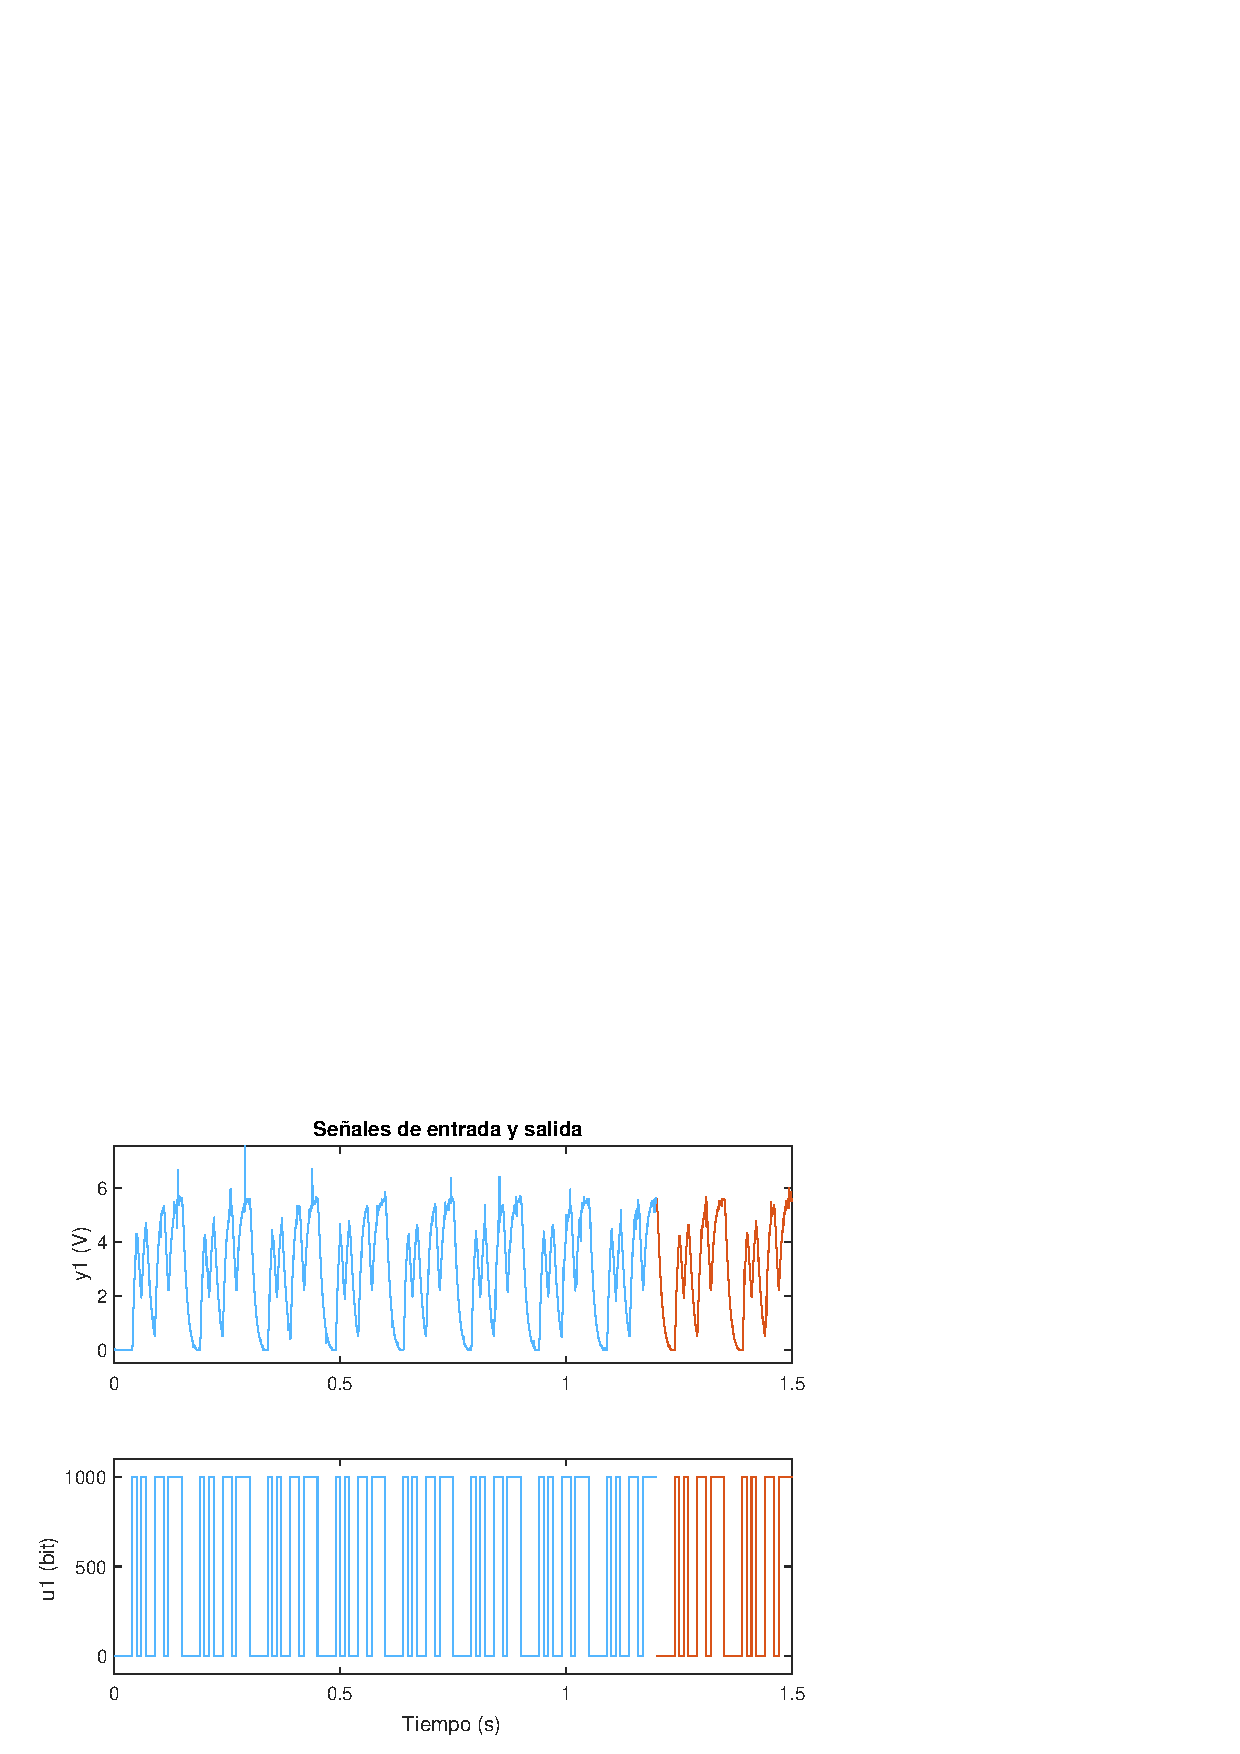
\includegraphics[height=6cm]{identificacion_io.png}
        %\vspace{-0.25cm}
        \caption{Vista completa de la señal de identificación.}
        \label{fig:identificacion_io_gral}
    \end{subfigure}
    \begin{subfigure}[b]{\textwidth}
        \centering
        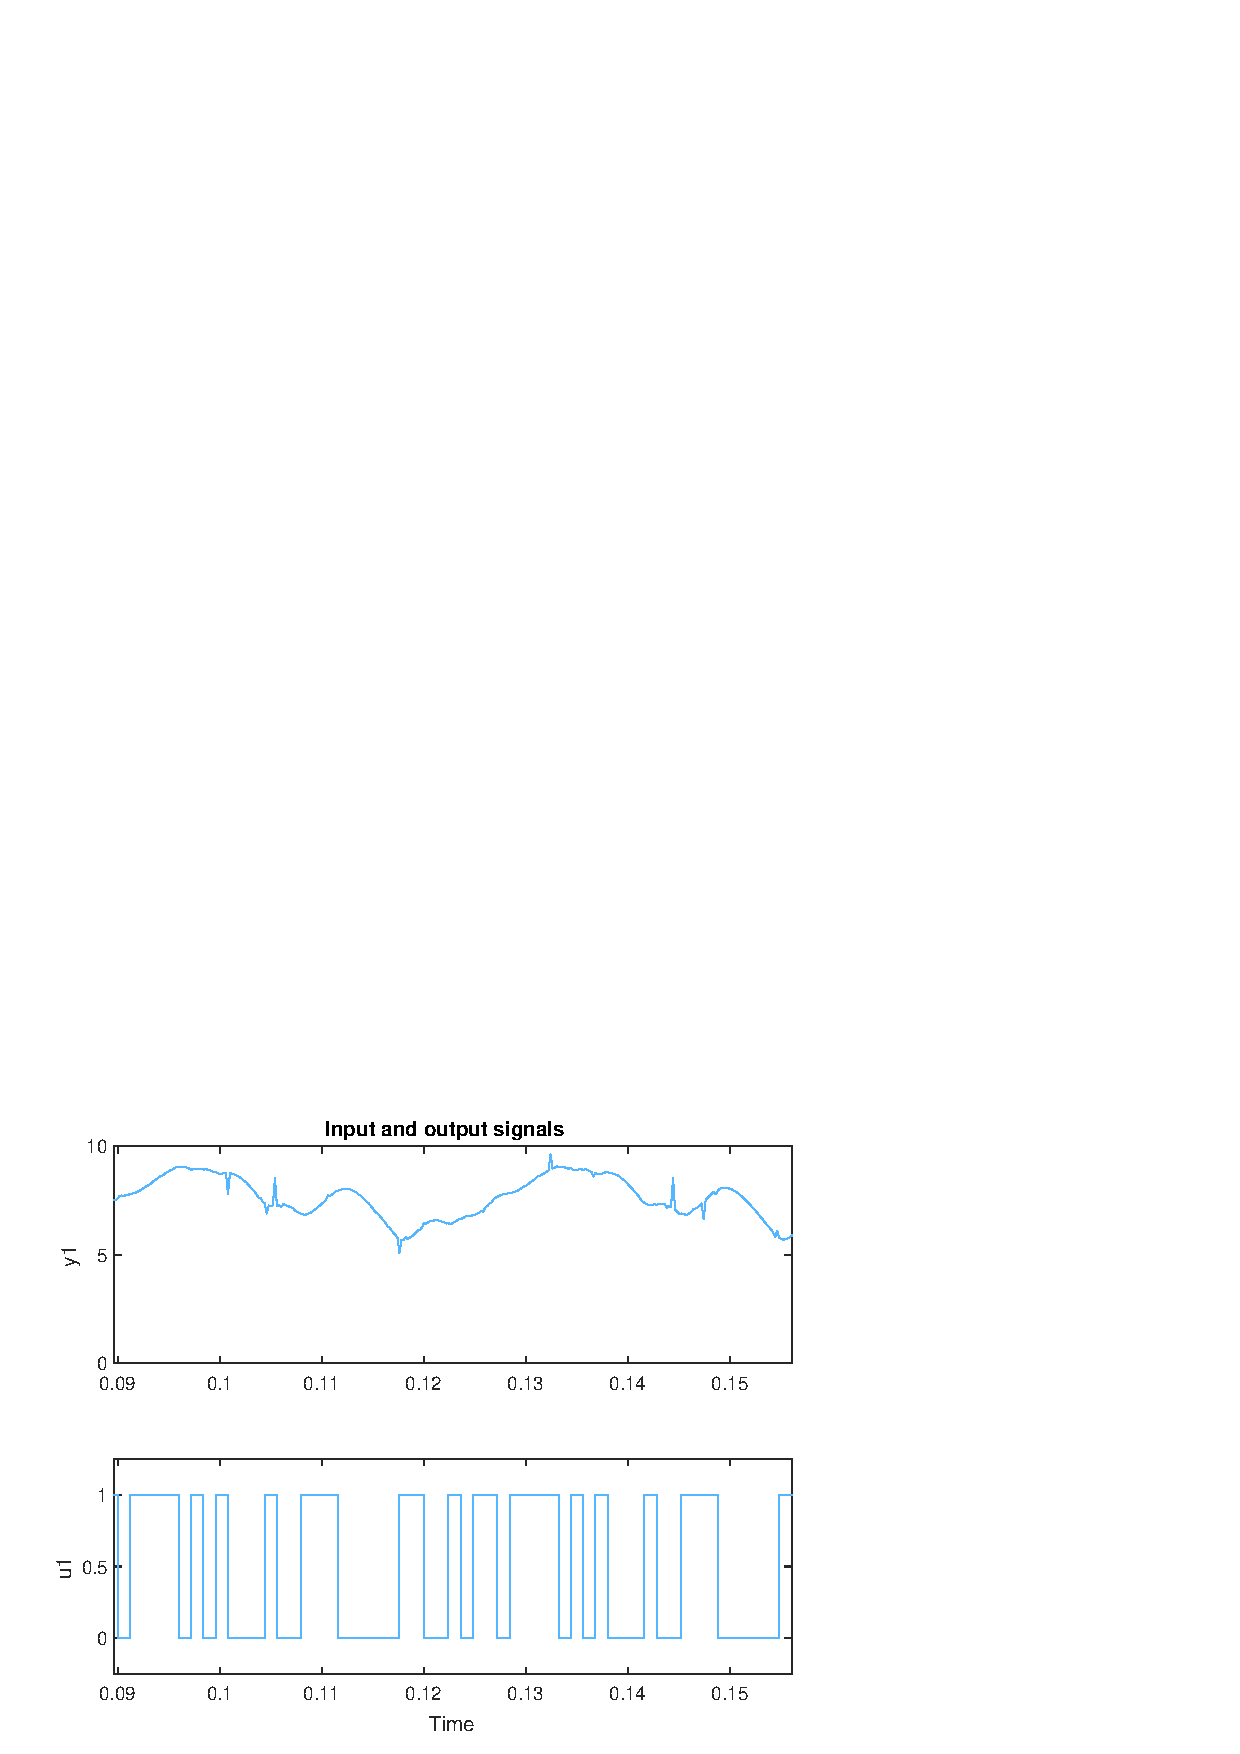
\includegraphics[height=6cm]{identificacion_zoom.png}
        %\vspace{-0.25cm}
        \caption{Vista acercada de la señal de identificación.}
        \label{fig:identificacion_io_zoom}
    \end{subfigure}

    \vspace{-0.25cm}
    \caption{Salida (arriba) y entrada (abajo) del sistema con la señal de identificación.}
    \label{fig:identificacion_io}
\end{figure}
\vspace{-0.5cm}

Se seleccionan los primeros 2455 valores (80\% de los valores totales) como la señal de evaluación
y los restantes 614 valores (20\% de los valores totales) como la señal de validación. Finalmente,
se estima un modelo en espacios de estado de orden 2 utilizando la función \textit{N4SID} del System Identification Toolbox:

\begin{figure}[H]
    \centering

    \begin{subfigure}[b]{\textwidth}
        \centering
        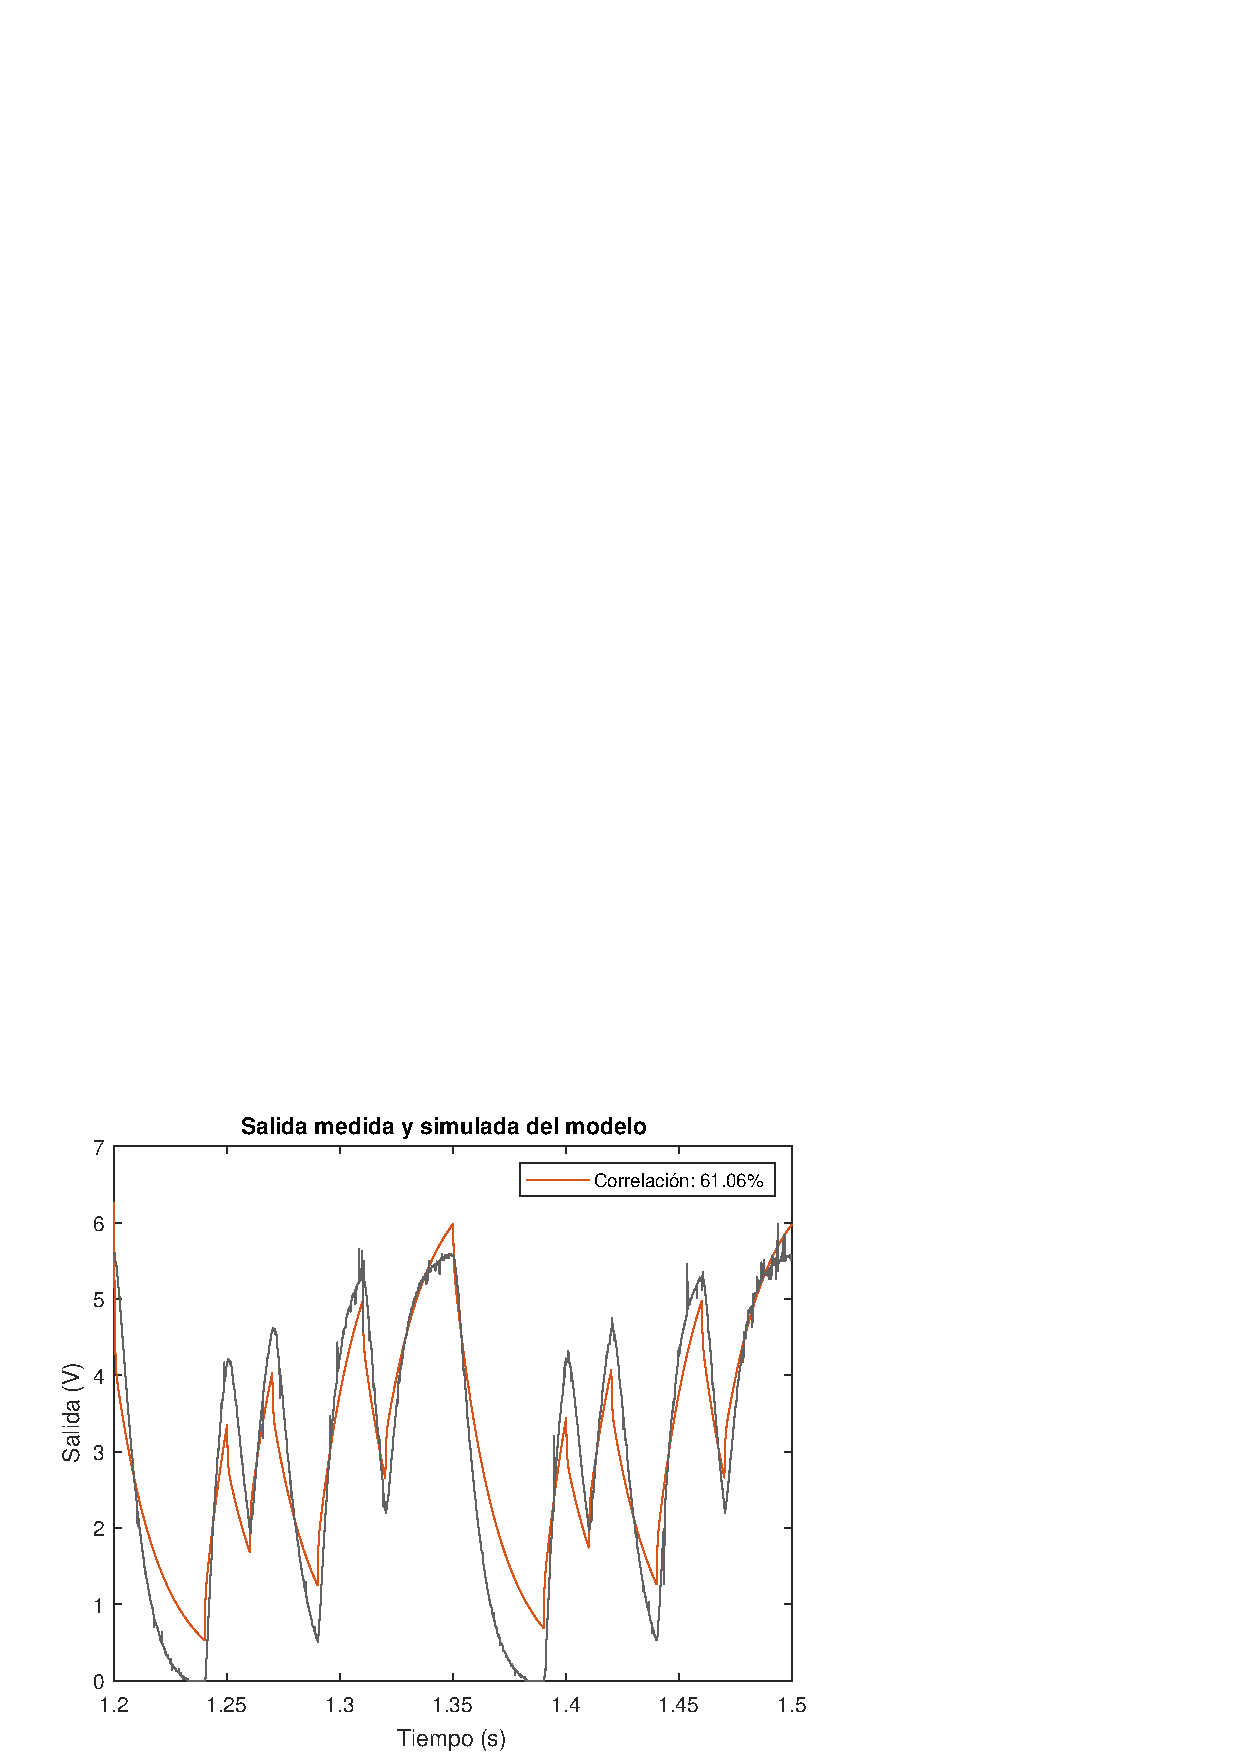
\includegraphics[width=10cm]{identificacion_comparacion.png}
        %\vspace{-0.25cm}
        \caption{Comparación del modelo estimado con la respuesta medida.}
        \vspace{0.25cm}
        \label{fig:identificacion_comparacio n}
    \end{subfigure}
    \begin{subfigure}[b]{\textwidth}
        \centering
        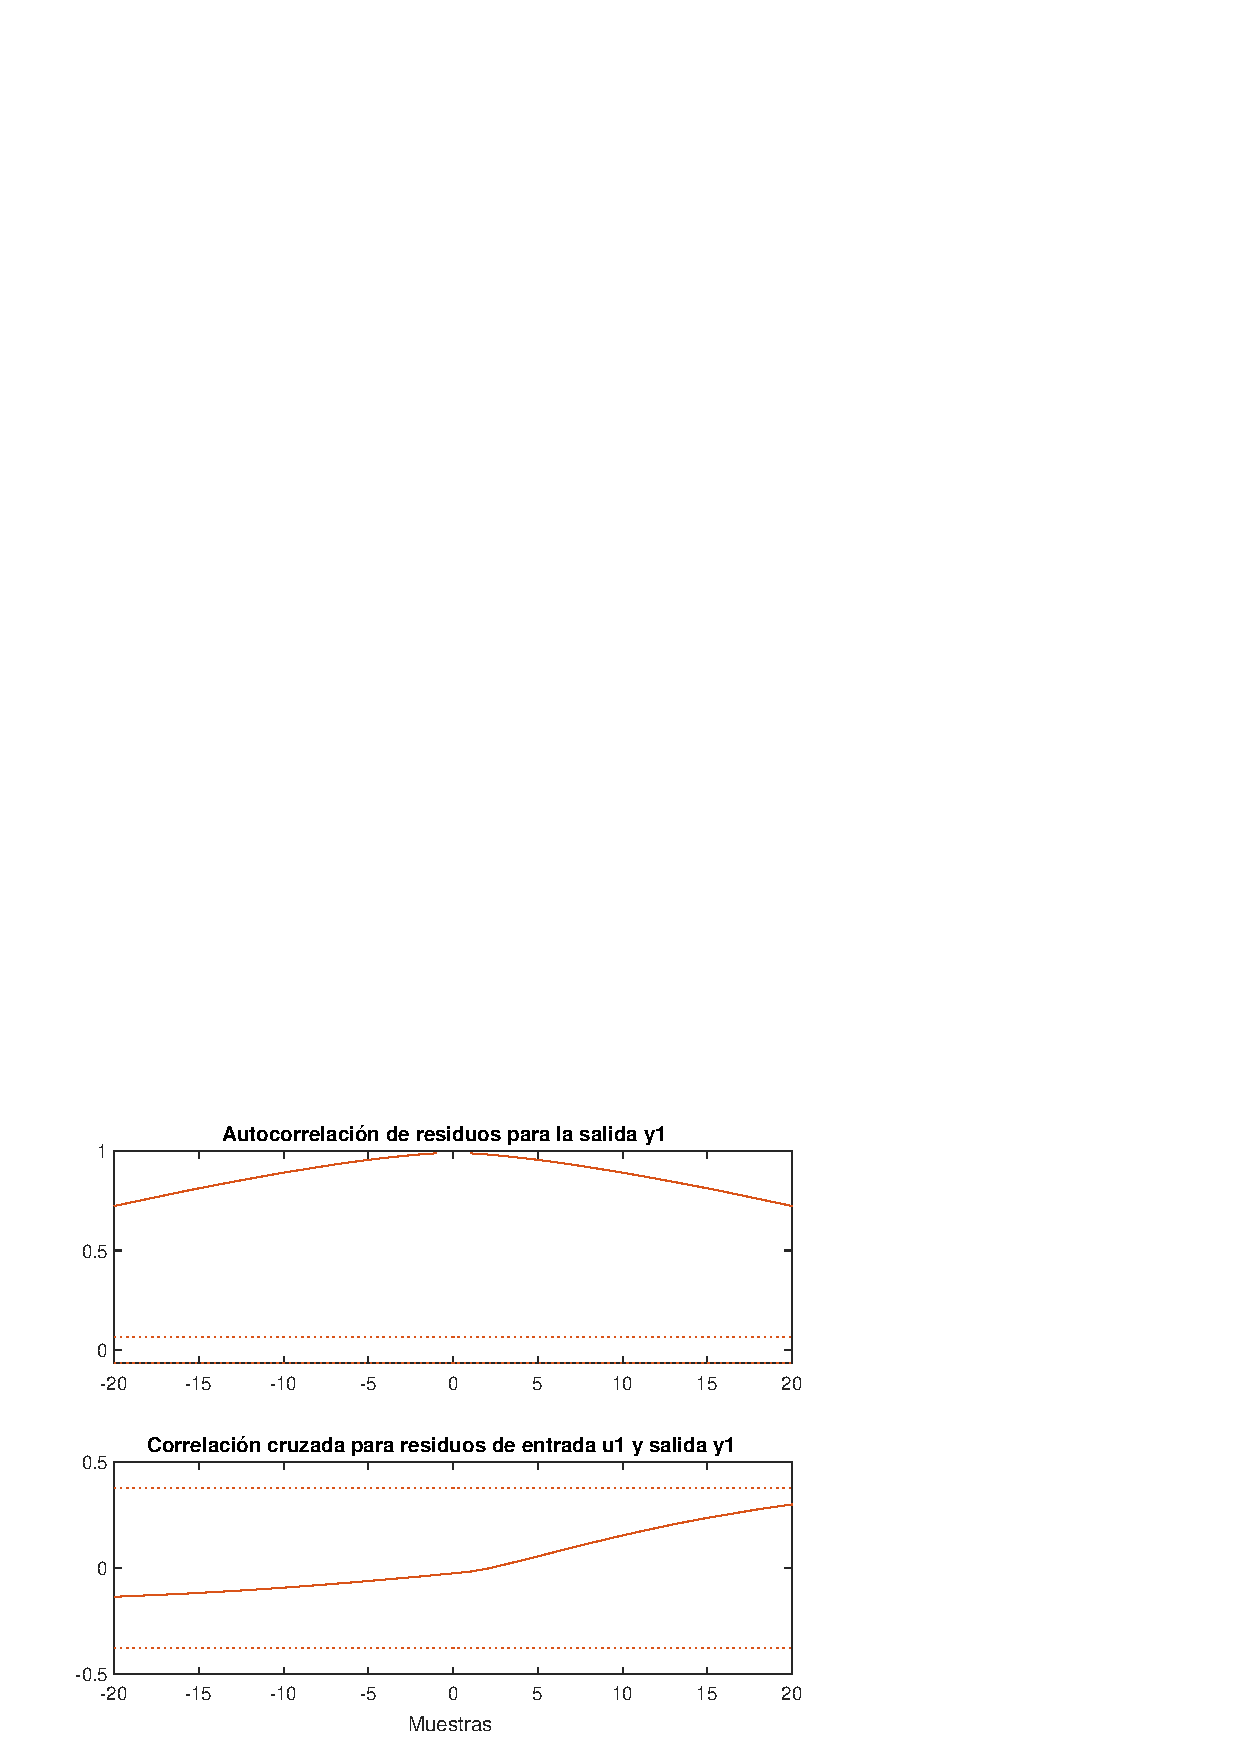
\includegraphics[width=10cm]{identificacion_residuos.png}
        %\vspace{-0.25cm}
        \caption{Análisis residual del modelo estimado.}
        \label{fig:identificacion_residuos}
    \end{subfigure}

    \vspace{-0.25cm}
    \caption{Resultados de la estimación del modelo del sistema.}
    \label{fig:identificacion_resultados}
\end{figure}
\vspace{-0.5cm}

Como se puede observar en la Figura \ref{fig:identificacion_resultados}, el modelo estimado coincide
con la respuesta medida del sistema (señal de evaluación) en un 73,39\%. Respecto a la señal de 
validación, coincide en un 65,8\%. Además, el análisis residual del modelo estimado
demuestra un buen resultado en la autocorrelación de residuales para la salida y un resultado
satisfactorio para la correlación cruzada de residuales entre la entrada y la salida.

El modelo estimado en espacios de estado es el siguiente:

\vspace{-0.5cm}
\begin{equation}
    \begin{cases}
        \begin{bmatrix}
            \dot{x_1}\\
            \dot{x_2}
        \end{bmatrix}
        =
        \begin{bmatrix}
            -213.1  &   279.1\\
            2819    &   -1.178\times 10^4
        \end{bmatrix}
        \cdot
        \begin{bmatrix}
            x_1 \\
            x_2
        \end{bmatrix}
        +
        \begin{bmatrix}
            -28.98 \\
            294,4
        \end{bmatrix}
        \cdot
        u 
        +
        \begin{bmatrix}
            -11.92 \\
            -95.37
        \end{bmatrix}
        \cdot
        e
        \\
        y =
        \begin{bmatrix}
            -56.54 & 4.834
        \end{bmatrix}
        \cdot
        \begin{bmatrix}
            x_1 \\
            x_2
        \end{bmatrix}
        +
        e

    \end{cases}
\end{equation}

El mismo se puede representar en función de transferencia luego de transformarlo mediante MATLAB:

\vspace{-0.5cm}
\begin{equation}
    H(s) = \dfrac{3062\ s + 1.456 \times 10^7}{s^2 + 1.199 \times 10^4\ s + 1.722 \times 10^6}
\end{equation}
\vspace{-0.5cm}

La planta discretizada mediante retención de orden cero (zoh), con un tiempo de muestreo de 200
microsegundos es:

\vspace{-0.5cm}
\begin{equation}
    H(z) = \dfrac{0.3798\ z - 0.1602}{z^2 - 1.065\ z + 0.09091}
\end{equation}
\vspace{-0.5cm}

A continuación se grafican las respuestas al impulso y al escalón, el mapa de polos y ceros y el lugar
geométrico de las raíces.

\begin{figure}[H]
    \centering

    \begin{subfigure}[b]{0.49\textwidth}
        \centering
        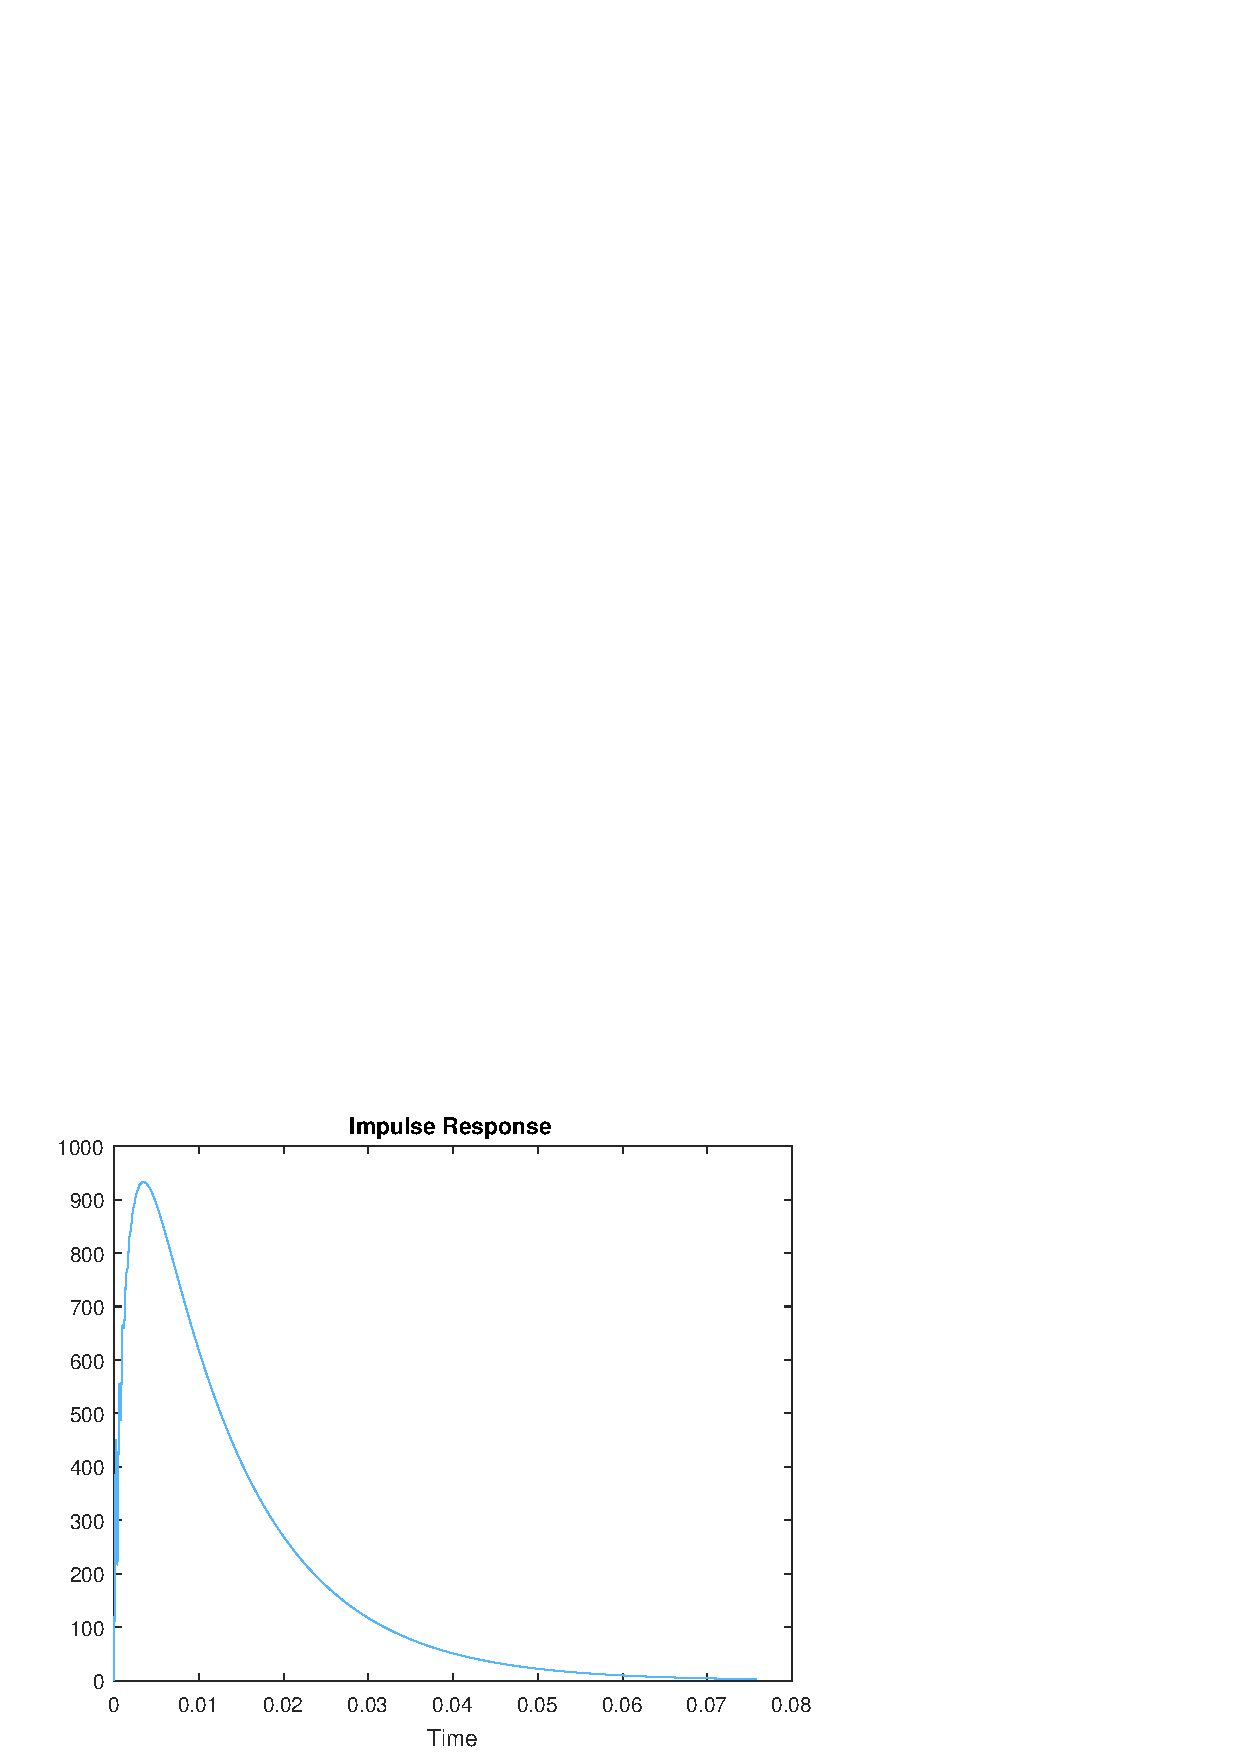
\includegraphics[width=\textwidth]{estimado_impulse.png}
        %\vspace{-0.25cm}
        \caption{Respuesta al impulso.}
        \label{fig:estimado_impulse}
    \end{subfigure}
    \begin{subfigure}[b]{0.49\textwidth}
        \centering
        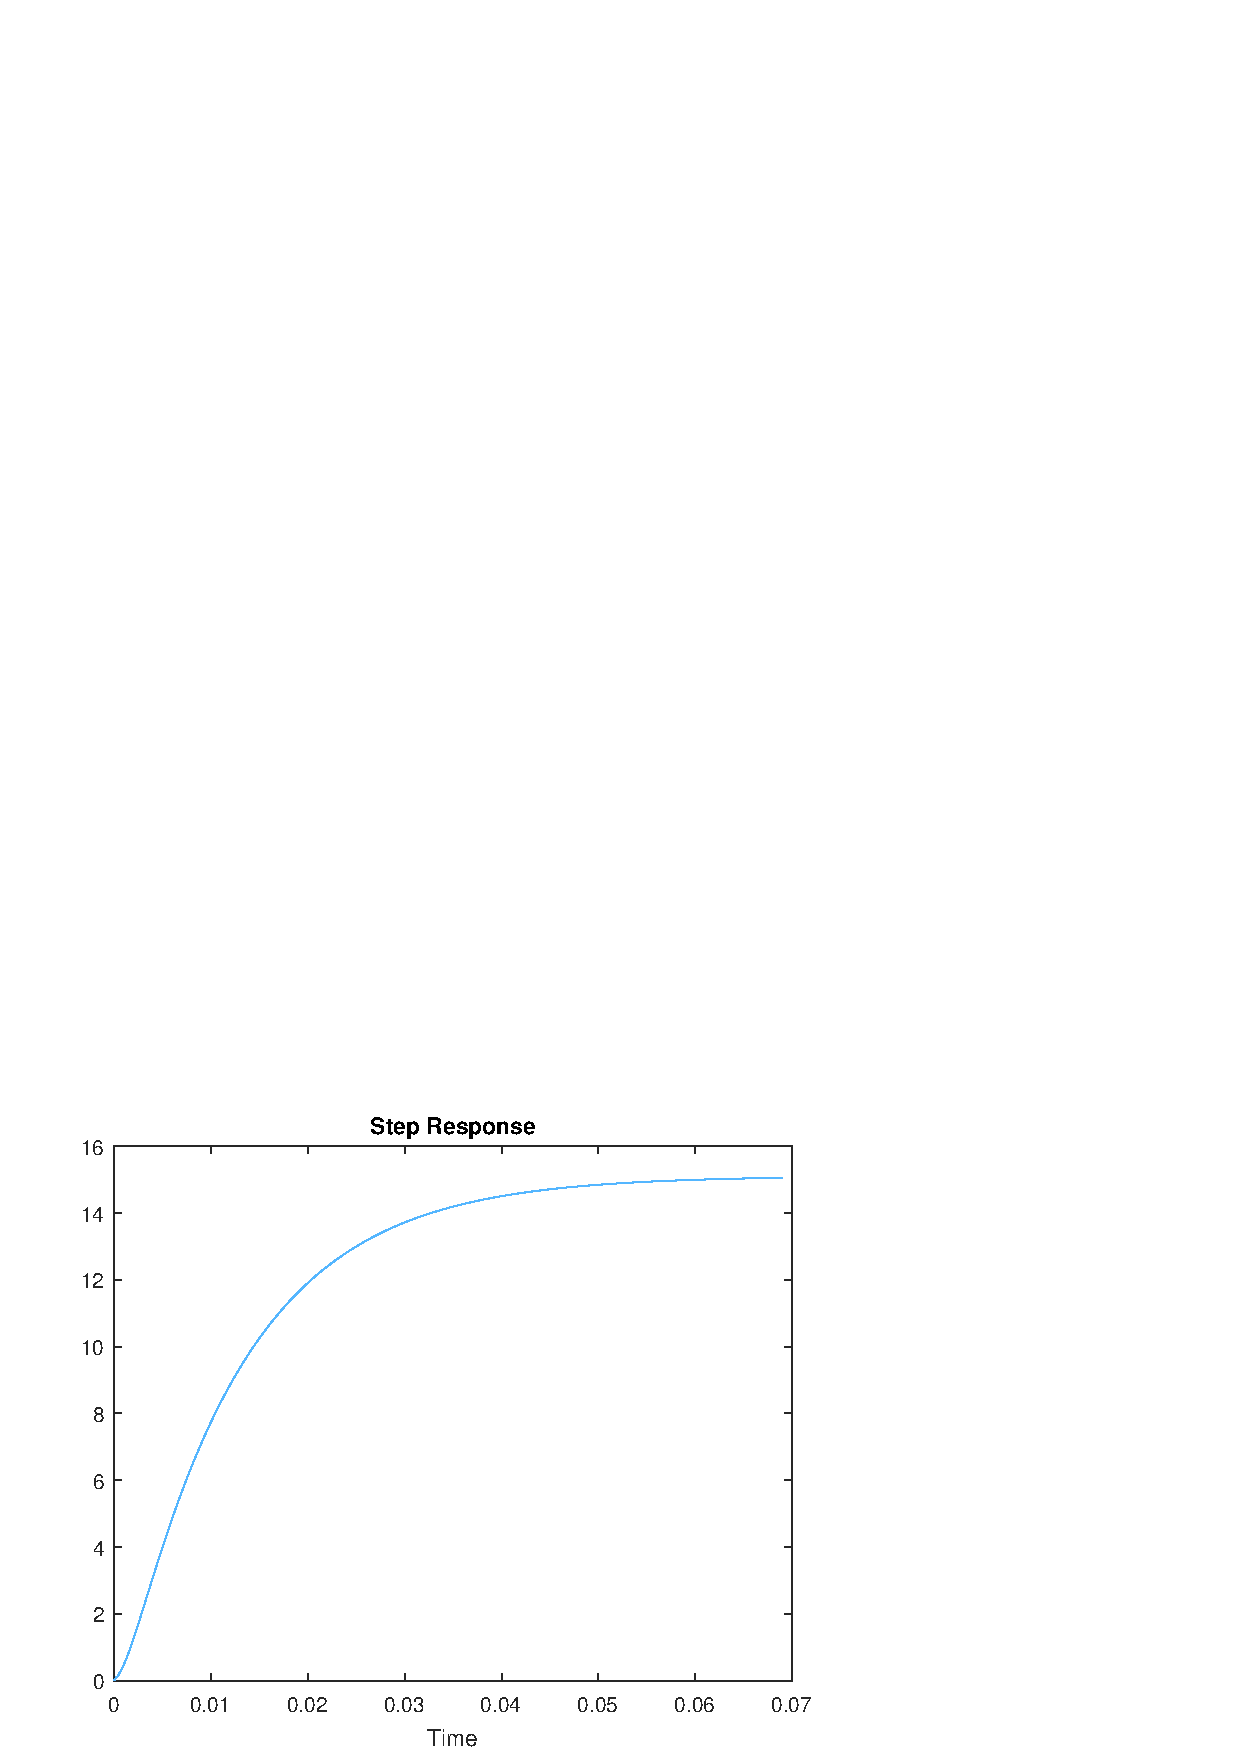
\includegraphics[width=\textwidth]{estimado_step.png}
        %\vspace{-0.25cm}
        \caption{Respuesta al escalón.}
        \label{fig:estimado_step}
    \end{subfigure}

    \vspace{-0.25cm}
    \caption{Análisis de la respuesta temporal del sistema estimado.}
    \label{fig:estimado_respuestas}
\end{figure}
\vspace{-0.5cm}

\begin{figure}[H]
    \centering

    \begin{subfigure}[b]{0.49\textwidth}
        \centering
        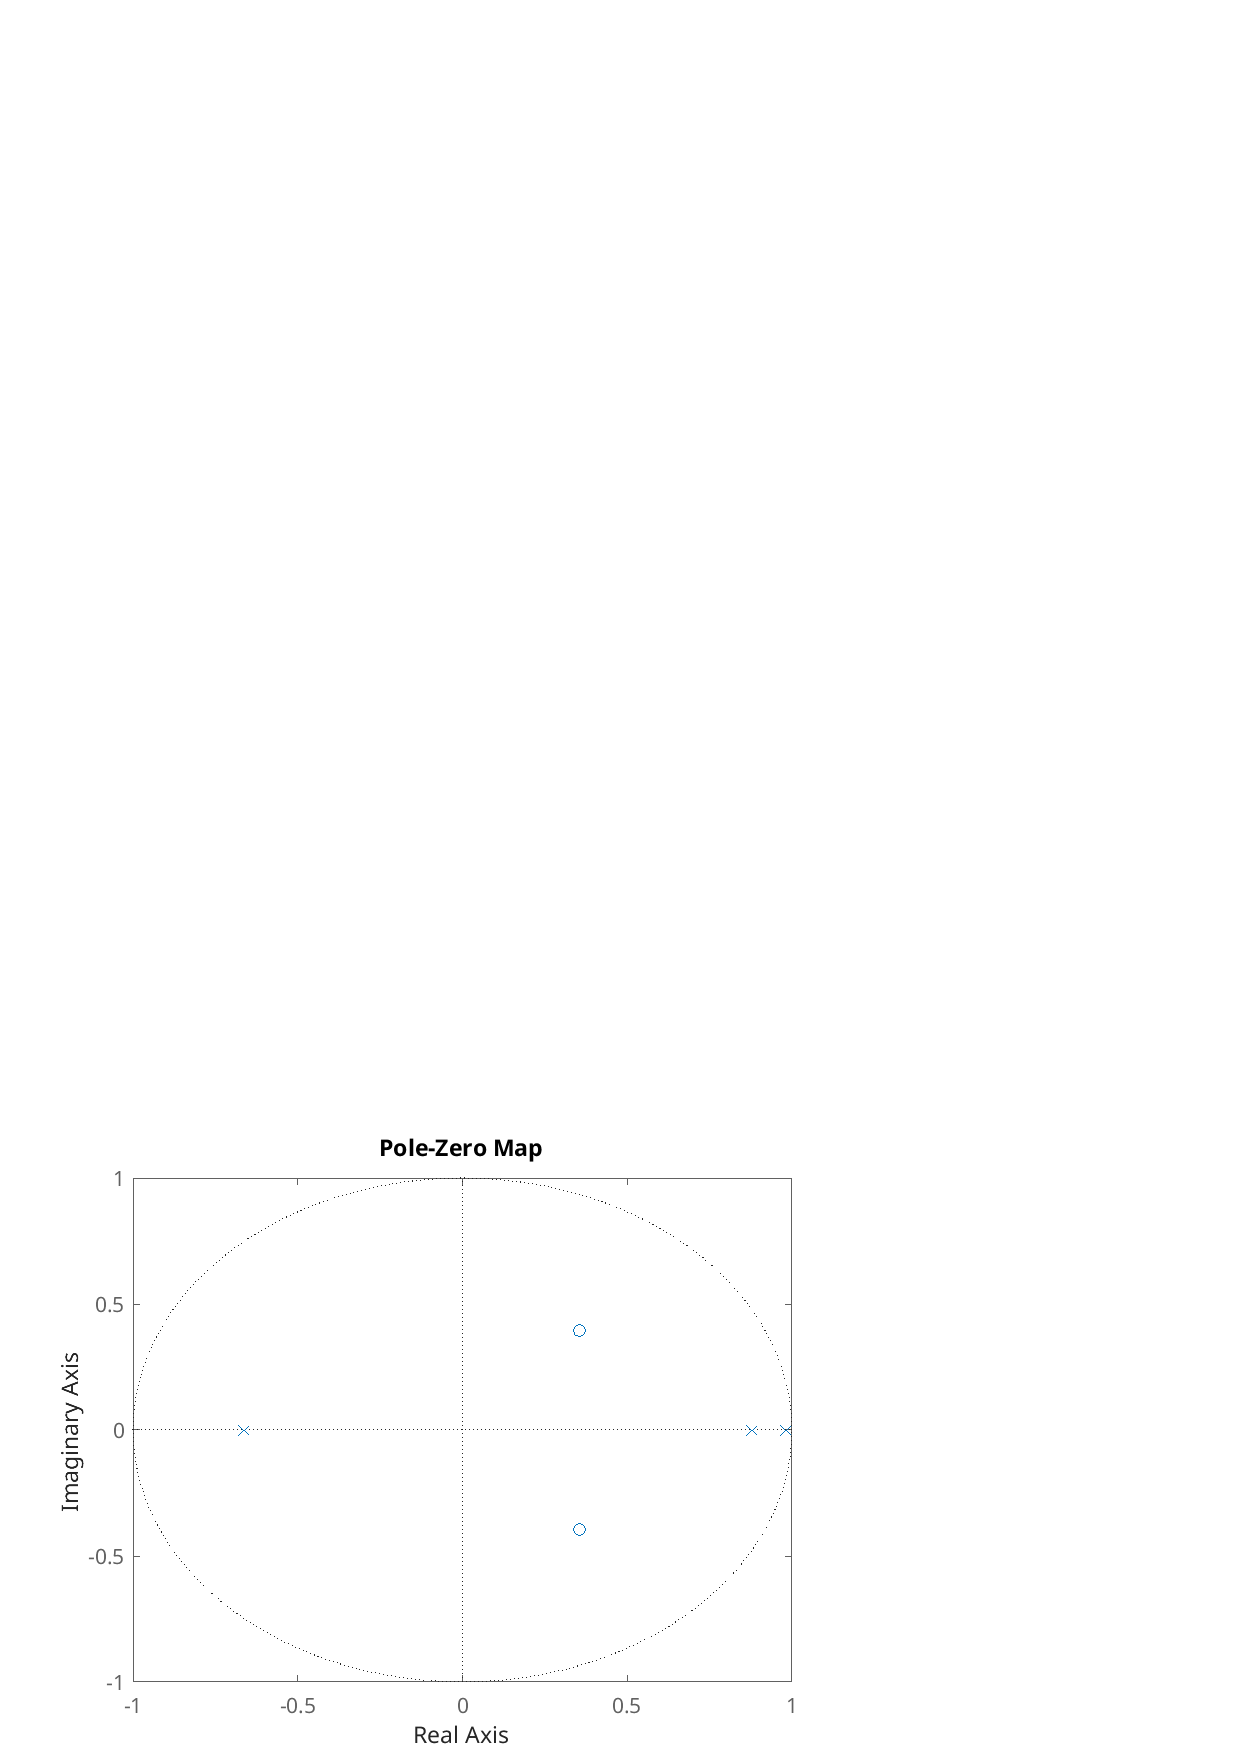
\includegraphics[width=\textwidth]{estimado_pzmap.png}
        %\vspace{-0.25cm}
        \caption{Mapa de polos y ceros.}
        \label{fig:estimado_pzmap}
    \end{subfigure}
    \begin{subfigure}[b]{0.49\textwidth}
        \centering
        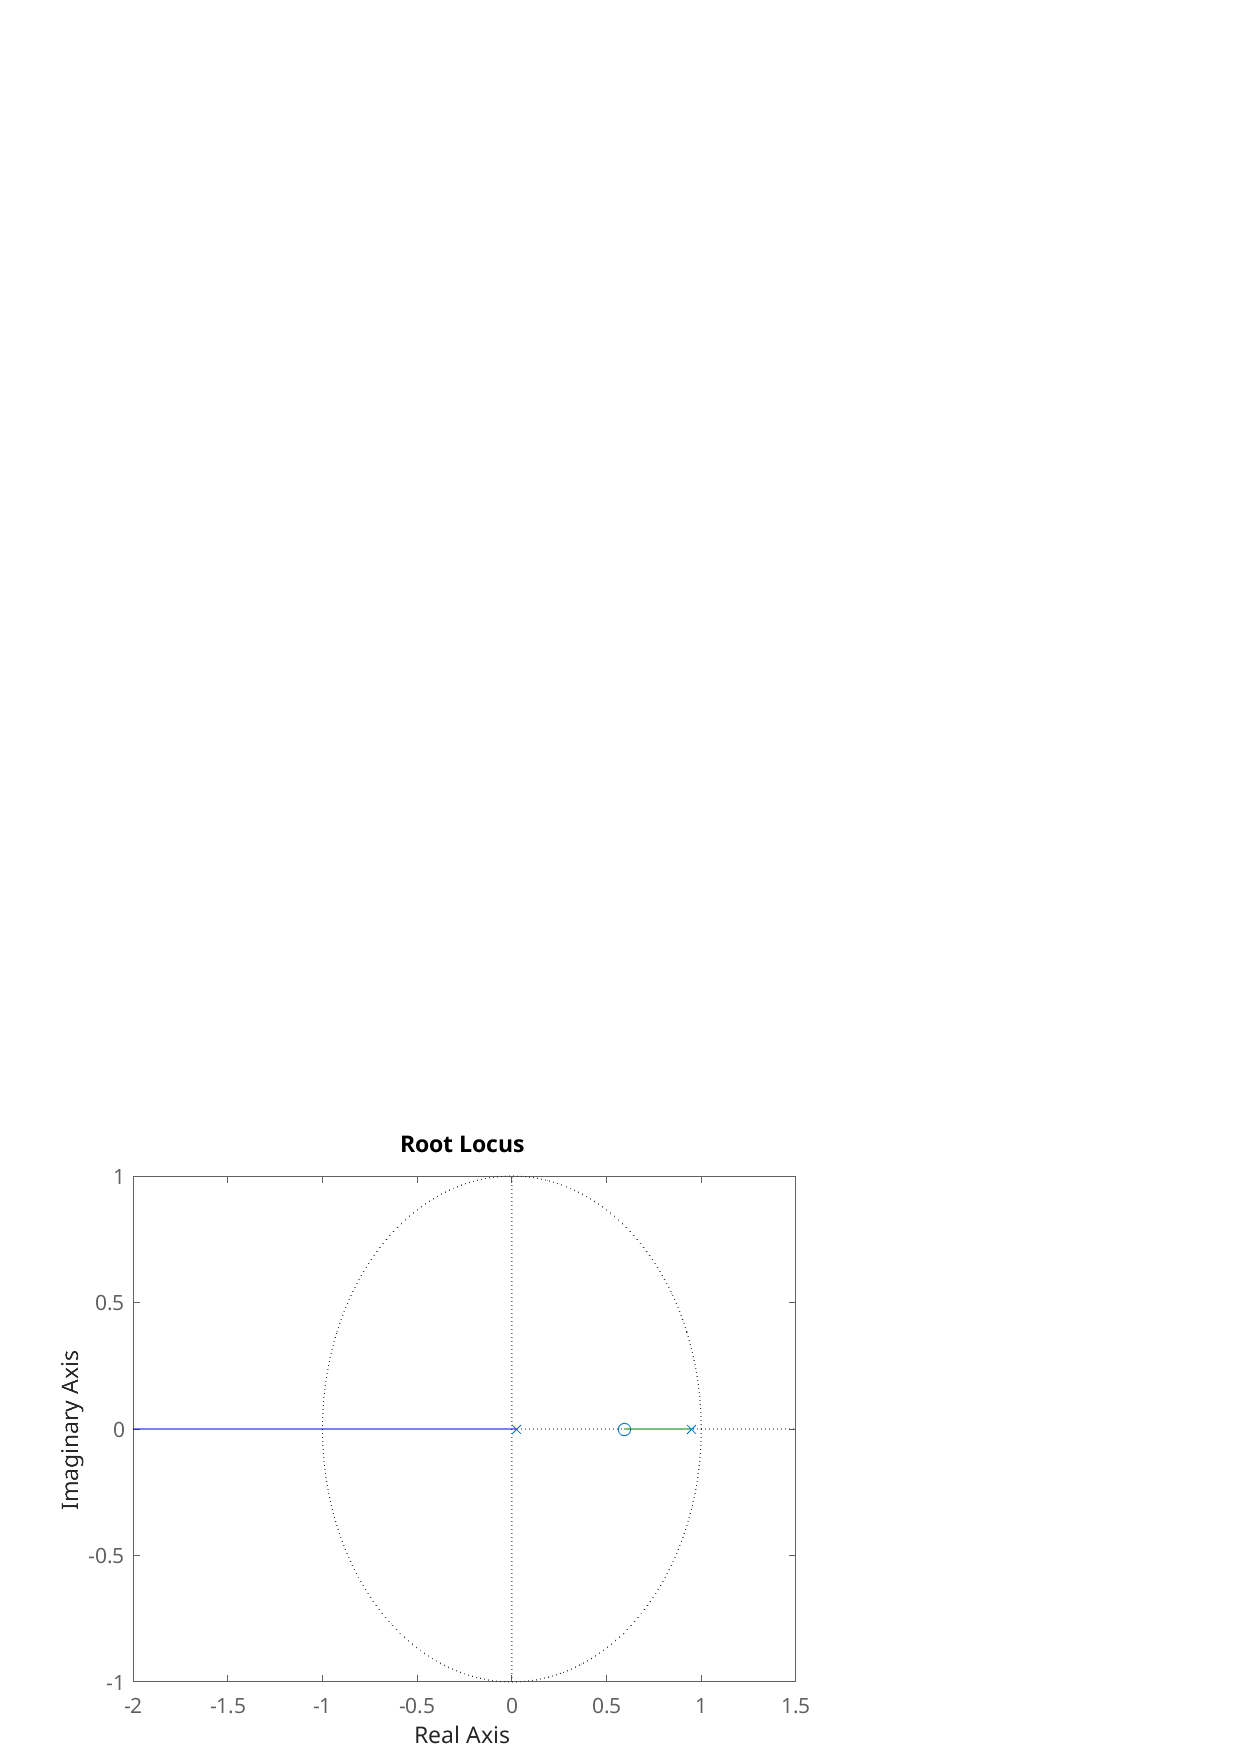
\includegraphics[width=\textwidth]{estimado_rlocus.png}
        %\vspace{-0.25cm}
        \caption{Lugar geométrico de las raíces.}
        \label{fig:estimado_rlocus}
    \end{subfigure}

    \vspace{-0.25cm}
    \caption{Análisis de la respuesta temporal del sistema estimado.}
    \label{fig:estimado_estabilidad}
\end{figure}
\vspace{-0.5cm}

La respuesta al impulso del sistema converge a cero cuando el tiempo tiende al infinito.
En la respuesta al escalon, el sistema converge a un valor.
La ubicación de polos y el lugar geométricos de las raices estan ubicados dentro 
del circulo unitario en el plano z. Debido a estas caracteristicas se determina que el sistema 
es estable.

    \newpage
    \section*{\large{CONCLUSIÓN}}
\vspace{-0.35cm}
\justifying

Conclusión aquí.

    \newpage
    \renewcommand{\refname}{\large REFERENCIAS}
    \begin{minipage}{0.96\textwidth}
    \printbibliography
    \end{minipage}

\end{document}